%================================================
%	PACKAGES AND THEMES
%================================================
\documentclass[aspectratio=169,xcolor=dvipsnames]{beamer}

\usetheme{SimplePlusAIC}

\usepackage{hyperref}
\usepackage{graphicx} % Allows including images
\usepackage{booktabs} % Allows the use of \toprule, \midrule and  \bottomrule in tables
\usepackage{svg} % Allows using svg figures
\usepackage{tikz}
\usepackage{makecell}
\newcommand*{\defeq}{\stackrel{\text{def}}{=}}
\usepackage{setspace}
\usepackage[T1]{fontenc}
\usepackage[french]{babel}
\usepackage{helvet}
\usepackage{textgreek}
\usepackage{amsmath,amssymb}
\usepackage{bm}
\usepackage{ragged2e}
\usepackage{xfrac}
% \usepackage[nice]{nicefrac}
\usepackage[loose]{units}
\usepackage{braket}
\usepackage{physics}
\usepackage{gensymb}

\usepackage{verbatim}
\usepackage{fancyvrb}
\usepackage{diagbox}

\usetikzlibrary{arrows}
\usetikzlibrary[patterns]

%-- For subfigures
\usepackage{subcaption}

%\setbeamertemplate{blocks}[rounded][shadow] % block options

\usepackage[svgnames,table]{xcolor}
\arrayrulecolor{black}
\setlength{\arrayrulewidth}{0.20mm}
\renewcommand{\arraystretch}{1.40}  % stretch tables row size

\usepackage{blkarray}
\usepackage{dsfont}

\usepackage{eurosym}
\usepackage{multicol}

%================================================
% MATH COMMANDS
%================================================
\newcommand{\R}{\mathbb{R}}
\renewcommand{\P}{\mathbb{P}}
\newcommand\indep{\protect\mathpalette{\protect\independenT}{\perp}}
\def\independenT#1#2{\mathrel{\rlap{$#1#2$}\mkern2mu{#1#2}}}

\newcommand{\argmin}{argmin}
%================================================
% Stuff for R code
%================================================

\usepackage{minted}
%================================================
% Pause après équation
%================================================
\newcommand{\pauseq}{\vspace*{-\baselineskip}\pause}
%================================================
% FontAwesome
\usepackage{fontawesome5}
%================================================

%================================================
%	TITLE PAGE
%================================================
\title[short title]{ECFG932 : Techniques avancées en analyse sensorielle} 
%\subtitle{Subtitle}

\author[Surname]{Guillaume Franchi}
\institute[CBI]{Cursus Ingénieur $3^{\text{ème}}$ année}

\date{\textcolor{nyublue}{JAR : Just About  Right}}


%================================================
%	BEGIN DOCUMENT 
%================================================



\begin{document}

%------------------------------------------------
%	TITLE SLIDE
%------------------------------------------------
\begin{frame}[plain]

    \titlepage
    
\end{frame}

%------------------------------------------------
%	OUTLINE SLIDE
%------------------------------------------------
%\begin{frame}[plain]
%
%    \frametitle{Plan du cours} 
%    %\framesubtitle{~}
%
%    \begin{spacing}{1.2}
%        \tableofcontents[hideallsubsections]
%    \end{spacing}
%    
%\end{frame}
%------------------------------------------------
%	SLIDE PRE-REQUIS
%------------------------------------------------

\begin{frame}[plain]

\textcolor{nyubluedarker}{{\Large \faCogs \ \textbf{Pré-requis}}}
	\begin{itemize}
	\item Test de Student.
	\item Analyse en Composantes Principales (ACP).
	\item Analyse Factorielle des Correspondances (AFC)
	\end{itemize}
	
\medskip

	\textcolor{nyubluedarker}{{\Large \faChalkboardTeacher \ \textbf{Enseignement}}}
	\begin{itemize}
	\item Cours : $\approx$ 45min.
	\item Travaux pratiques : $\approx$ 3h00.
	\end{itemize}	

\end{frame}



%~~~~~~~~~~~~~~~~~~~~~~~~~~~~~~~~~~~~~~~~~~~~~~~~
\section{Contexte et Objectifs}
%~~~~~~~~~~~~~~~~~~~~~~~~~~~~~~~~~~~~~~~~~~~~~~~~

%------------------------------------------------
%	NEW SLIDE
%------------------------------------------------
\begin{frame}[plain]

\vfill

\begin{center}
{\huge \textcolor{nyubluedark}{\textbf{1. Contexte et Objectifs}}}
\end{center}

\vfill

\end{frame}

%------------------------------------------------
%	NEW SLIDE
%------------------------------------------------
\begin{frame}
	\begin{exampleblock}{\textbf{Exemple}}
		\begin{itemize}
		\item On a fait goûter 8 fromages à pâte pressée à un panel de 72 consommateurs :
		\setlength{\columnsep}{0.02cm}
			\begin{multicols}{4}
			\begin{itemize}
			\item Beaufort (B);
			\item Cantal 1 (C1);
			\item Cantal 2 (C2);
			\item Comté (CE);
			\item Emmental (E);
			\item Morbier (M);
			\item Reblochon (R);
			\item St-Nectaire (S).
			\end{itemize}
			\end{multicols}
		\item Les consommateurs ont noté ces fromages par :
			\begin{itemize}
			\item une \textbf{note hédonique} d'appréciation globale (échelle de 1 à 9);
			\item une évaluation de 9 attributs sensoriels, selon une \textbf{échelle JAR} en 5 points :
			\setlength{\columnsep}{-0.8cm}
				\begin{multicols}{3}
				\begin{itemize}
				\item[$\triangleright$] Couleur;
				\item[$\triangleright$] Consistance toucher;
				\item[$\triangleright$] Intensité odeur;
				\item[$\triangleright$] Intensité goût;
				\item[$\triangleright$] Goût fruité;
				\item[$\triangleright$] Goût salé;
				\item[$\triangleright$] Fermeté texture;
				\item[$\triangleright$] Crémeux texture;
				\item[$\triangleright$] Intensité arrière-goût.
				\end{itemize}
				\end{multicols}
			\end{itemize}
		\begin{scriptsize}
			\emph{Exemple :}
				
				\begin{tabular}{cccccc}
				 & Vraiment pas assez salé & Pas assez salé & Juste bien & Trop salé & Vraiment trop salé \\
				 \hline
				Goût salé & $\square$ & $\square$ & $\square$ & $\square$ & $\square$ 
				\end{tabular}
			\end{scriptsize}
		\end{itemize}
	\end{exampleblock}
\end{frame}

%------------------------------------------------
%	NEW SLIDE
%------------------------------------------------
\begin{frame}
	\begin{exampleblock}{\textbf{Exemple (suite)}}
\begin{scriptsize}
\begin{center}
\begin{tabular}{llrlllllllll}
  \hline
Conso & Produit & Liking & Couleur & Cons & Odeur & Int\_g & Fr\_g & Sel\_g & Ferm & Crem & Int\_ag \\ 
  \hline
33001 & Comté &   3 & 2 & 4 & 2 & 2 & 2 & 3 & 2 & 2 & 2 \\ 
33001 & Morbier &   4 & 2 & 2 & 2 & 4 & 2 & 4 & 2 & 4 & 4 \\ 
33001 & Beaufort &   2 & 4 & 5 & 1 & 1 & 1 & 3 & 5 & 2 & 1 \\ 
33001 & Reblochon &   3 & 3 & 1 & 3 & 2 & 2 & 3 & 2 & 3 & 2 \\ 
33001 & Cantal1 &   4 & 2 & 4 & 2 & 2 & 2 & 5 & 4 & 2 & 2 \\ 
33001 & Emmental &   1 & 3 & 4 & 1 & 2 & 2 & 3 & 4 & 2 & 2 \\ 
33001 & Cantal2 &   7 & 2 & 4 & 1 & 3 & 3 & 4 & 3 & 3 & 3 \\ 
33001 & St-Nectaire &   5 & 3 & 2 & 1 & 2 & 2 & 3 & 3 & 3 & 2 \\ 
33010 & Morbier &   5 & 3 & 2 & 3 & 4 & 2 & 3 & 3 & 3 & 4 \\ 
   \hline
\end{tabular}
\end{center}

\underline{Source :} Thèse CIFRE Oniris  d'Alexiane Luc, 2022, \emph{Evaluation de la perception des consommateurs à l'aide du protocole
sensoriel Free JAR : une nouvelle méthodologie de collecte d'analyse
statistique des données}.
\end{scriptsize}
	\end{exampleblock}
\end{frame}

%------------------------------------------------
%	NEW SLIDE
%------------------------------------------------
\begin{frame}
	
	\vfill

\textcolor{nyubluedarker}{\faBullseye \ \textbf{Objectifs :}}
		
	\medskip		
		
	\begin{itemize}
	\item[\faCogs] Déterminer les liens entre les notes d'appréciation globale et les évaluations sensorielles JAR.
	\item[\faCogs] Identifier les défauts d'un produit.
	\item[\faCogs] Déterminer les relations entre les attributs JAR.
	\item[\faCogs] Situer un produit par rapport aux autres.
	\end{itemize}
	
	\vfill	
	
\end{frame}

%------------------------------------------------
%	NEW SLIDE
%------------------------------------------------
\begin{frame}
\textcolor{nyubluedarker}{\faChartBar \ \textbf{Cartographie interne des préférences}}

\begin{center}
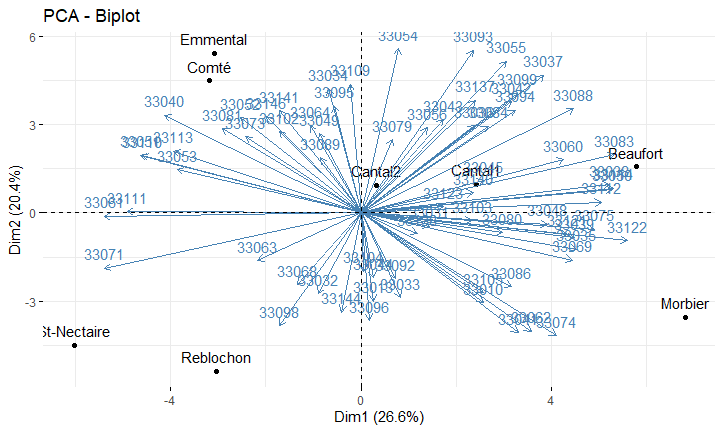
\includegraphics[scale=0.5]{cart_interne.png}
\end{center}

\textcolor{nyubluedarker}{\faLightbulb[regular]} Les goûts des consommateurs sont très hétérogènes.

\medskip

\textcolor{nyubluedarker}{\faLightbulb[regular]} Les produit \og Comté \fg{} et \og Emmental \fg{} d'une part, et \og Morbier \fg{} d'autre part, sont des produits segmentants.  

\end{frame}

%------------------------------------------------
%	NEW SLIDE
%------------------------------------------------
\begin{frame}
\textcolor{nyubluedarker}{\faChartBar \ \textbf{Représentations graphiques (1/3)}}

	\medskip

	\begin{figure}
	\centering
	\begin{subfigure}{0.5\textwidth}
	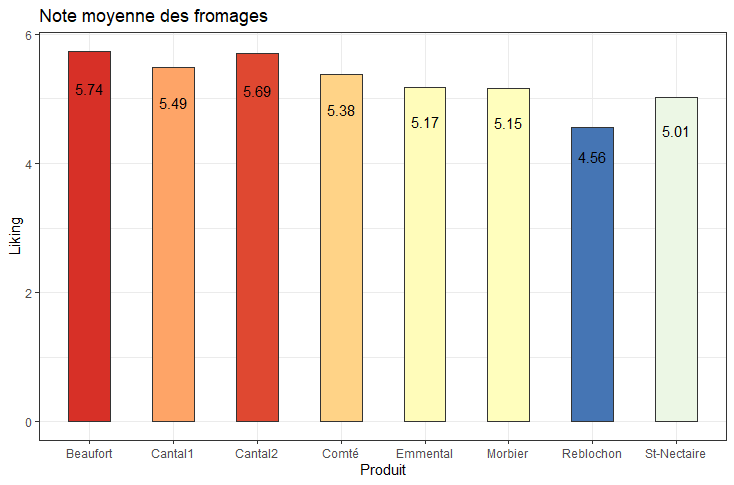
\includegraphics[width=\textwidth]{note_fromages.png}
	\end{subfigure}~
	\begin{subfigure}{0.5\textwidth}
	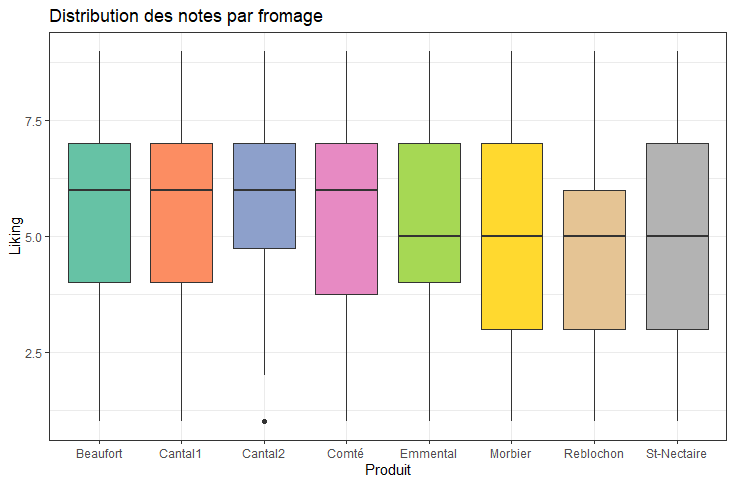
\includegraphics[width=\textwidth]{boxplots_notes_fromages.png}
	\end{subfigure}
	\end{figure}

\end{frame}

%------------------------------------------------
%	NEW SLIDE
%------------------------------------------------

\begin{frame}
\textcolor{nyubluedarker}{\faChartBar \ \textbf{Représentations graphiques (2/3)}}

	\begin{figure}
	\centering
	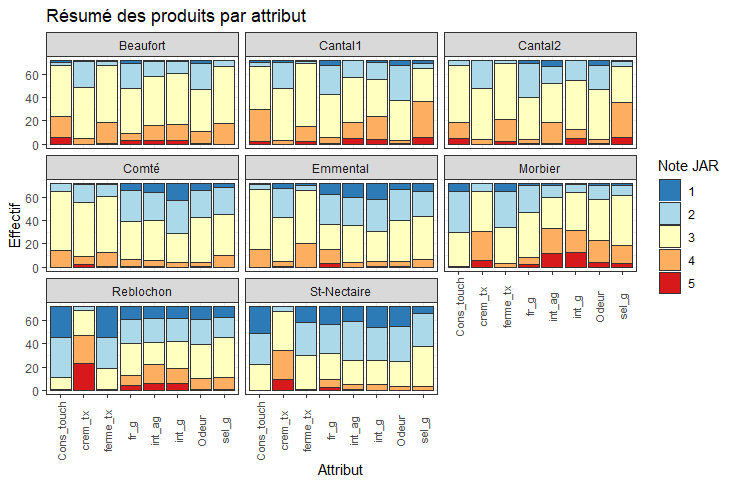
\includegraphics[width=0.8\textwidth]{distrib_notesJAR_attribut.png}
	\end{figure}

\end{frame}

%------------------------------------------------
%	NEW SLIDE
%------------------------------------------------

\begin{frame}
\textcolor{nyubluedarker}{\faChartBar \ \textbf{Représentations graphiques (3/3)}}

	\begin{figure}
	\centering
	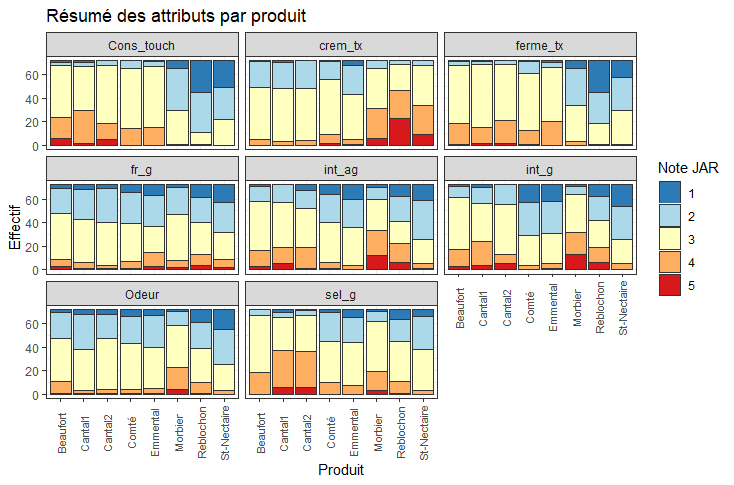
\includegraphics[width=0.8\textwidth]{distrib_notesJAR_produit.png}
	\end{figure}

\end{frame}

%~~~~~~~~~~~~~~~~~~~~~~~~~~~~~~~~~~~~~~~~~~~~~~~~
\section{Analyses sur échelles JAR discontinues}
%~~~~~~~~~~~~~~~~~~~~~~~~~~~~~~~~~~~~~~~~~~~~~~~~

%------------------------------------------------
%	NEW SLIDE
%------------------------------------------------
\begin{frame}[plain]

\vfill

\begin{center}
{\huge \textcolor{nyubluedark}{\textbf{2. Analyses sur échelles JAR discontinues}}}
\end{center}

\vfill

\end{frame}

%------------------------------------------------
%	NEW SLIDE
%------------------------------------------------
\begin{frame}
	\begin{block}{\textbf{Echelles JAR}}
		\begin{itemize}
		\item L'échelle JAR la plus utilisée pour noter un attribut du produit est une échelle de réponse discontinue structurée.
		\item Il est demandé à chaque individu de cocher la case correspondant le mieux à son avis sur l'attribut considéré.
		\item La valeur idéale est placée au centre de l'échelle, qui comporte en général 3,5,7 ou 9 points. 
		\end{itemize}
	\end{block}
	
	\begin{figure}
		\centering
		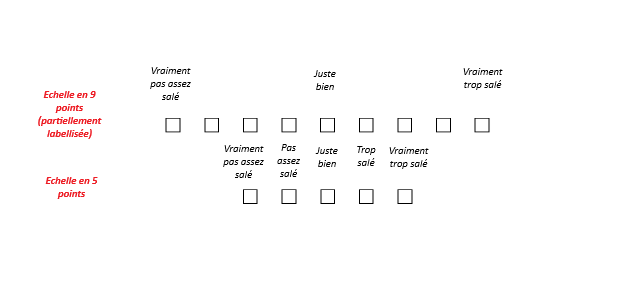
\includegraphics[width=0.7\textwidth]{expl_echelles_dis_JAR.png}
	\end{figure}
\end{frame}

%------------------------------------------------
%	NEW SLIDE
%------------------------------------------------
\begin{frame}
	\begin{exampleblock}{\textbf{Remarques}}
		\begin{itemize}
		\item L'évaluation sensorielle des attributs du produit s'accompagne d'une note hédonique d'appréciation globale du produit. \emph{(\textbf{liking})}.
		\item En général, chaque individu évalue plusieurs produits.
		\item La taille d'échantillon préconisée est d'au moins 75 consommateurs \emph{(Source : SFAS, 2022)}.
		\end{itemize}
	\end{exampleblock}
\end{frame}

%------------------------------------------------
%	NEW SLIDE
%------------------------------------------------
\begin{frame}
	\begin{block}{\textbf{Périmètre d'analyse}}
		\begin{itemize}
		\item L'objectif principal est de mesurer l'impact d'un attribut sur l'appréciation générale.
		\item Deux solutions :
			\begin{itemize}
			\item Conduire les analyses par produit.
			\item Conduire les analyses tous produits confondus.
			\end{itemize}
		\end{itemize}
	\end{block}
	
	\begin{exampleblock}{\textbf{Remarque}}
		\begin{itemize}
		\item Les méthodes d'analyse sont identiques dans les deux cas, seules les interprétations diffèrent.
		\item Dans l'exemple qui suit, on ne fait que l'analyse du produit \og Beaufort \fg{}. 
		\end{itemize}

	\end{exampleblock}
\end{frame}

%------------------------------------------------
%	NEW SLIDE
%------------------------------------------------
\begin{frame}
\textcolor{nyubluedarker}{\faCogs \ \textbf{Pré-traitement :}} Les différents items de l'échelle sont regroupés en 3 catégories: \og Pas assez \fg{}, \og JAR \fg{} ou \og Trop \fg{}.
		\begin{figure}
		\centering
		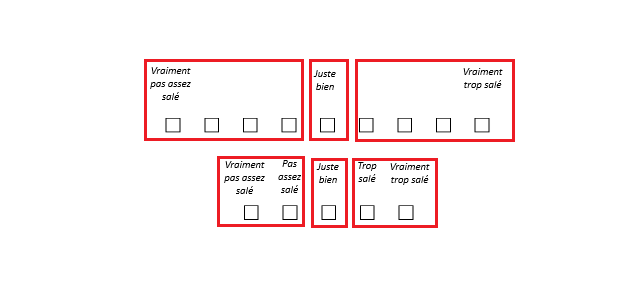
\includegraphics[width=0.6\textwidth]{group_echelles.png}
		\end{figure}
	On calcule alors la fréquence de chacun de ces groupes :
		\begin{itemize}
		\item \og Pas assez \fg{}  salé : 0.0694
		\item \og JAR \fg{}  salé : 0.681
		\item \og Trop \fg{} salé : 0.25
		\end{itemize}	

\end{frame}

%------------------------------------------------
%	NEW SLIDE
%------------------------------------------------
\begin{frame}

\textcolor{nyubluedarker}{\faCogs \ \textbf{Pénalité \emph{(Mean drop)} :}}

	\begin{itemize}
	\item On calcule ensuite les moyennes des appréciations globales pour chaque groupe ainsi défini.
		\begin{itemize}
		\item \og Pas assez \fg{}  salé : 3.20
		\item \og JAR \fg{}  salé : 6.37
		\item \og Trop \fg{} salé : 4.72
		\end{itemize}
	\item Les deux effets sur la moyenne d'un attribut sont alors
		\begin{itemize}
		\item \og Pas assez \fg{} salé : Moyenne \og JAR \fg{} salé $-$ Moyenne \og Pas assez \fg{} salé
			\[6.37-3.20 = 3.17.\]
		\item \og Trop \fg{} salé : Moyenne \og JAR \fg{} salé $-$ Moyenne \og Trop \fg{} salé
			\[6.37-4.72 = 1.65.\]
		\end{itemize}
	\end{itemize}
		
\end{frame}

%------------------------------------------------
%	NEW SLIDE
%------------------------------------------------
\begin{frame}
	\begin{exampleblock}{\textbf{Remarques}}
		\begin{itemize}
		\item Les catégories d’attribut JAR avec un pourcentage de consommateurs dans les catégories \og Pas assez \fg{}  ou \og Trop \fg{} inférieur à 20\% ne doivent pas être considérées \emph{(même si les logiciels les présentent)}.
		\item Il n'est pas souhaitable de conserver une catégorie avec moins de 15 sujets en absolu, même si le critère de 20\% est respecté.
		\end{itemize}
	\emph{Source : SFAS, 2022}
	\end{exampleblock}
\end{frame}

%------------------------------------------------
%	NEW SLIDE
%------------------------------------------------
\begin{frame}

\textcolor{nyubluedarker}{\faChartBar \ \textbf{Représentation graphique} :}

	\begin{figure}
	\centering
	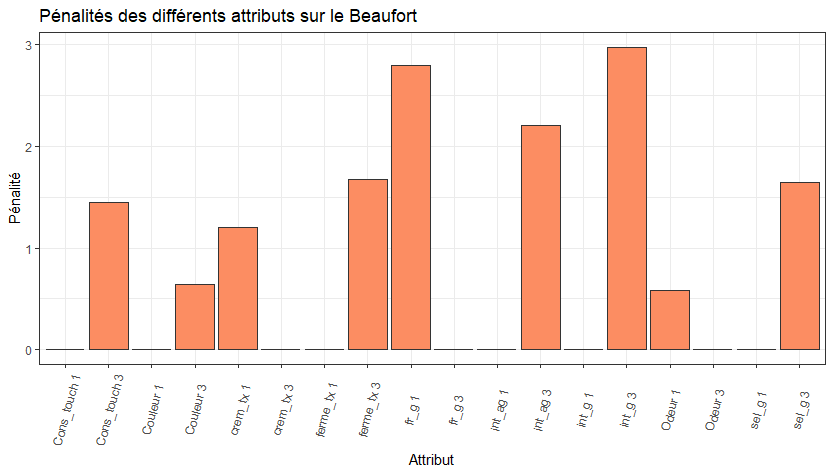
\includegraphics[width = 0.8\textwidth]{penalites_beaufort.png}
	\end{figure}

\end{frame}

%------------------------------------------------
%	NEW SLIDE
%------------------------------------------------
\begin{frame}

\textcolor{nyubluedarker}{\faCogs \ \textbf{Significativité statistique} :}

Les effets sur la moyenne peuvent être statistiquement testés en effectuant un \textbf{test de Student}.

\medskip

	\begin{exampleblock}{\textbf{Exemple}}
	Comparons la moyenne d'appréciation globale des consommateurs ayant trouvé le Beaufort \og Trop salé \fg{} par rapport à la moyenne donnée par ceux l'ayant trouvé \og JAR \fg{} salé.
	\end{exampleblock}
\end{frame}

%------------------------------------------------
%	NEW SLIDE
%------------------------------------------------
\begin{frame}	
	\begin{exampleblock}{\textbf{Exemple (suite)}}
	On note :
		\begin{itemize}
		\item $m_3$ et $m_2$ les moyennes théoriques des deux groupes;
		\item $n_3 = 18$ et $n_2 = 49$ les effectifs des deux groupes;
		\item $\overline{x}_3 = 4.72$ et $\overline{x}_2 = 6.37$ les moyennes des deux groupes;
		\item $S_3^2 = \frac{1}{n_3} \sum_{i=1}^{n_3} (x_i^{(3)} - \overline{x}_3)^2$ et $S_2^2 = \frac{1}{n_2} \sum_{i=1}^{n_2} (x_i^{(2)} - \overline{x}_2)^2 $ les variances empiriques des deux groupes.
		\end{itemize}
	
	\medskip		
		
	On teste $H_0$ : $m_3 = m_2$ contre $H_1$ : $m_3 < m_2$. Sous les hypothèses adéquates, on a 
		\[
		T = \dfrac{ \sqrt{n_2+n_3-2} \left(\overline{x}_3-\overline{x}_2 \right)}{\left( n_3 S_3^2 + n_2 S_2^2 \right) \left( 1/n_3 + 1/n_2 \right)} \sim \mathcal{T}_{n_3+n_2-2}.
		\]
	On rejette $H_0$ au seuil de 5\% si $T < q_{0.05}$, le quantile d'ordre 0.05 de la loi $\mathcal{T}_{n_3+n_2-2}$.   
	\end{exampleblock}

\end{frame}

%------------------------------------------------
%	NEW SLIDE
%------------------------------------------------
\begin{frame}	
	\begin{exampleblock}{\textbf{Exemple (suite)}}
	Ici, on obtient $T \approx -2.87$ et $q_{0.05} \approx -1.67 $ le quantile d'ordre 0.05 de la loi $\mathcal{T}_{65}$.
	
	\medskip
	
	On rejette donc $H_0$.
	
	\medskip
	
	Par ailleurs, la $p$-value calculée ici vaut $p \approx 2.75\times 10^{-3}$.
	\end{exampleblock}
	
	\begin{exampleblock}{\textbf{Remarque}}
	La loi de Student permet également de construire des intervalles de confiance pour la pénalité théorique $m_2-m_3$.
	\end{exampleblock}
\end{frame}
%------------------------------------------------
%	NEW SLIDE
%------------------------------------------------
\begin{frame}
	\begin{scriptsize}
	\begin{itemize}
	\item Sur l'exemple du beaufort, et sur les catégories pertinentes, on obtient les résultats suivants.	
	\end{itemize}

	\begin{center}
	\begin{tabular}{ccccccc}
  \hline
Attribut & Effectif & Fréquence & Moyenne & Pénalité & $p$-value & Significativité à 5\% \\ 
  \hline 
Cons\_touch\_3 &  24 & 33.33 & 4.92 & 1.45 & $5.06\times 10^{-3}$ & Oui \\ 
Couleur\_3 &  25 & 34.72 & 5.36 & 0.64 & $0.13$ & Non \\ 
Odeur\_1 &  25 & 34.72 & 5.36 & 0.58 & $0.17$ & Non \\  
crem\_tx\_1 &  23 & 31.94 & 5.04 & 1.21 & $2.00\times 10^{-2}$ & Oui \\ 
ferme\_tx\_3 &  19 & 26.39 & 4.53 & 1.68 & $2.60\times 10^{-3}$ & Oui \\ 
fr\_g\_1 &  24 & 33.33 & 4.21 & 2.79 & $2.31\times 10^{-8}$ & Oui \\  
int\_ag\_3 &  16 & 22.22 & 4.12 & 2.21 & $1.83\times 10^{-4}$ & Oui \\ 
int\_g\_3 &  17 & 23.61 & 3.94 & 2.97 & $1.2\times 10^{-8}$ & Oui \\  
sel\_g\_3 &  18 & 25.00 & 4.72 & 1.65 & $2.75\times 10^{-3}$ & Oui \\ 
   \hline
	\end{tabular}
	\end{center}
	\end{scriptsize}
\end{frame}

%------------------------------------------------
%	NEW SLIDE
%------------------------------------------------
\begin{frame}
	\begin{itemize}
	\item On peut représenter l'ensemble des pénalités \emph{(significatives ou non)} sur un graphique croisé ayant :
		\begin{itemize}
		\item en abscisse le pourcentage de consommateurs de chaque catégorie;
		\item en ordonnée la pénalité de la catégorie.
		\end{itemize}
	
	\begin{figure}
	\centering
	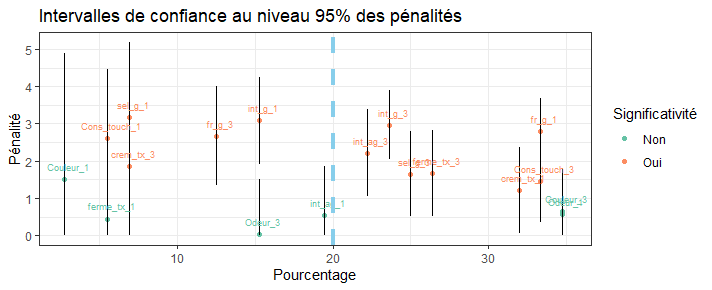
\includegraphics[width=0.8\textwidth]{conf_pen.png}
	\end{figure}
	\item On peut également ajouter les intervalles de confiance pour les pénalités.
	\end{itemize}
\end{frame}

%------------------------------------------------
%	NEW SLIDE
%------------------------------------------------
\begin{frame}
\textcolor{nyubluedarker}{\faCogs \ \textbf{Interprétation :}}

	En règle générale :
		\begin{itemize}
		\item Une catégorie \og Pas assez \fg{} ou \og Trop \fg{} est un point d'amélioration si le pourcentage est supérieur à 30\%;
		\item Une catégorie \og JAR \fg{} est un point fort si le pourcentage est supérieur à 60\%, avec une répartition équilibrée des deux autres catégories.  
		\end{itemize}
	\emph{Source : SFAS, 2022.}
	
	\begin{exampleblock}{\textbf{Exemple}}
	La salinité du beaufort ne peut pas être considérée comme un point fort :
		\begin{itemize}
		\item \og Pas assez \fg{} salé : 6.9\%;
		\item \og JAR \fg{} salé : 68.1\% 
		\item \og Trop \fg{} salé : 25\%. 
		\end{itemize}
	\end{exampleblock}
\end{frame}

%------------------------------------------------
%	NEW SLIDE
%------------------------------------------------
\begin{frame}
\textcolor{nyubluedarker}{\faCogs \ \textbf{La pénalité pondérée :}}

\vfill

	\begin{itemize}
	\item Elle est obtenue en multipliant la pénalité d'une appréciation JAR \og Trop \fg{} ou \og Pas assez \fg{} par la fréquence des consommateurs ayant choisi cette appréciation.
	\item Dans notre exemple, on a comme pénalités pondérées
		\begin{itemize}
		\item \og Pas assez \fg{} salé : $3.17\times0.0694 \approx 0.22$.
		\item \og Trop \fg{} salé : $1.65\times 0.25 \approx 0.41$.  
		\end{itemize}
	\end{itemize}

\vfill

\end{frame}

%------------------------------------------------
%	NEW SLIDE
%------------------------------------------------
\begin{frame}
\textcolor{nyubluedarker}{\textbf{A titre indicatif}}

\medskip

		\begin{itemize}
		\item Sur une échelle d'appréciation globale graduée de 1 à 9 :
		\begin{itemize}
		\item Si la pénalité pondérée est inférieure à 1 alors le défaut est considéré comme mineur.
		\item Si la pénalité pondérée est supérieure à 1 alors le défaut est considéré comme majeur.
		\end{itemize}
		\item Sur une échelle d'appréciation globale graduée de 1 à 6 :
		\begin{itemize}
		\item Si la pénalité pondérée est inférieure à 0.5 alors le défaut est considéré comme mineur.
		\item Si la pénalité pondérée est supérieure à 0.5 alors le défaut est considéré comme majeur.
		\end{itemize}
		\end{itemize}
\end{frame}

%------------------------------------------------
%	NEW SLIDE
%------------------------------------------------
\begin{frame}

\begin{exampleblock}{\textbf{Exemple}}
Dans notre exemple sur le beaufort, il n'y a aucun défaut majeur.
	\begin{center}
	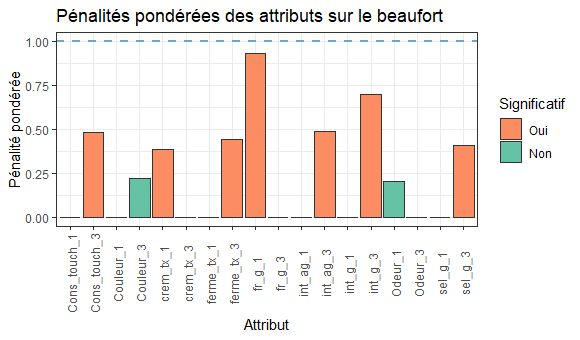
\includegraphics[scale=0.7]{pen_pond.png}
	\end{center}
\end{exampleblock}

\end{frame}

%~~~~~~~~~~~~~~~~~~~~~~~~~~~~~~~~~~~~~~~~~~~~~~~~
\section{Analyses sur échelles JAR continues}
%~~~~~~~~~~~~~~~~~~~~~~~~~~~~~~~~~~~~~~~~~~~~~~~~

%------------------------------------------------
%	NEW SLIDE
%------------------------------------------------
\begin{frame}[plain]

\vfill

\begin{center}
{\huge \textcolor{nyubluedark}{\textbf{3. Analyses sur échelles JAR continues}}}
\end{center}

\vfill

\end{frame}

%------------------------------------------------
%	NEW SLIDE
%------------------------------------------------
\begin{frame}

\textcolor{nyubluedarker}{\faCogs} Selon les études, il es parfois demandé au consommateur de noter chaque attribut sur une échelle \textbf{continue} \emph{(mesurée, par exemple, de 0 à 10cm)}.

	\begin{center}
	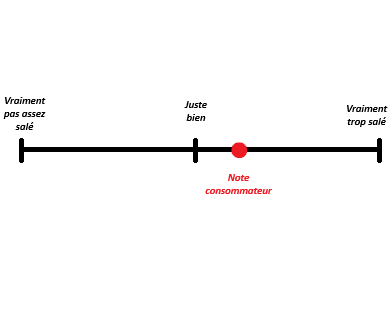
\includegraphics[scale=0.6]{ech_cont.png}
	\end{center}
\textcolor{nyubluedarker}{\faCogs} Chaque variable considérée est alors \textbf{quantitative} \emph{(ou numérique)}.
\end{frame}

%------------------------------------------------
%	NEW SLIDE
%------------------------------------------------
\begin{frame}
	\begin{exampleblock}{\textbf{Exemple}}
	\begin{scriptsize}
	Dans notre exemple des fromages, on pourrait avoir
	\begin{center}
\begin{tabular}{lrrrrrrrrrr}
  \hline
Produit & Liking & Couleur & Cons\_touch & Odeur & int\_g & fr\_g & sel\_g & ferme\_tx & crem\_tx & int\_ag \\ 
  \hline
CE & 2.90 & 4.20 & 6.20 & 3.90 & 3.90 & 3.90 & 5.30 & 3.90 & 4.20 & 4.10 \\ 
M & 4.00 & 4.10 & 4.10 & 4.10 & 6.30 & 4.10 & 6.40 & 3.80 & 6.30 & 6.00 \\ 
B & 2.30 & 5.80 & 7.40 & 3.40 & 3.50 & 3.20 & 5.10 & 7.00 & 3.90 & 3.30 \\ 
R & 3.00 & 5.10 & 3.10 & 4.80 & 4.40 & 4.30 & 5.20 & 3.90 & 4.80 & 3.90 \\ 
C1 & 4.00 & 4.00 & 6.00 & 4.20 & 4.00 & 4.00 & 7.20 & 6.30 & 3.90 & 3.70 \\ 
E & 1.30 & 5.10 & 6.20 & 3.30 & 3.70 & 4.10 & 5.30 & 6.00 & 4.20 & 4.20 \\ 
   \hline
\end{tabular}
	\end{center}
	\end{scriptsize}
	\end{exampleblock}
\end{frame}

%------------------------------------------------
%	NEW SLIDE
%------------------------------------------------
\begin{frame}
	\begin{block}{\textbf{Modèle ANOVA}}
		\begin{itemize}
		\item On effectue une \textbf{analyse de variance} pour chaque attribut, dans le but de les trier du moins au plus discriminant, \textbf{tous produits confondus}.
		\item Le modèle associé est :
			\[
			\mathbf{X}_{i,j}^{(k)} = \mu + \alpha_i^{(k)} + \beta_j^{(k)} + \varepsilon_{i,j}^{(k)}
			\]
		où
			\begin{itemize}
			\item $\mu$ est une constante \emph{(appréciation d'un produit de référence par un consommateur de référence)};
			\item $\mathbf{X}_{i,j}^{(k)}$ est la note du consommateur $i$ donnée au produit $j$ pour l'attribut $k$;
			\item $\alpha_i^{(k)}$ est un effet aléatoire du niveau $i$ du facteur \emph{consommateur} pour l'attribut $k$;
			\item $\beta_j^{(k)}$ est un effet fixe du niveau $j$ du facteur produit pour l'attribut $k$;
			\item $\varepsilon_{i,j}^{(k)}$ est une variable aléatoire résiduelle.
			\end{itemize}
		\end{itemize}
		
	\end{block}
\end{frame}

%------------------------------------------------
%	NEW SLIDE
%------------------------------------------------
\begin{frame}
	\begin{exampleblock}{\textbf{Remarques}}
	Dans le modèle 
		\[
		\mathbf{X}_{i,j}^{(k)} = \mu + \alpha_i^{(k)} + \beta_j^{(k)} + \varepsilon_{i,j}^{(k)}
		\]
		\begin{itemize}
		\item[\faCogs] Seuls l'effet fixe du produit et l'effet aléatoire du consommateur sont testés.
		
		\item[\faLightbulb] L'effet de l'interaction n'est pas testable, chaque consommateur n'ayant évalué un produit d'une seule fois.
		
		\item[\faCogs] Cette analyse globale ne permet pas de discerner les différences individuelles entre produits... Il se peut qu'un seul produit soit responsable d'un effet produit.
		
		\item[\faLightbulb] Dans ce cas, on peut effectuer un test de comparaison multiple des moyennes \emph{(comme le test de Duncan)}.
		\end{itemize}
	\end{exampleblock}
\end{frame}

%------------------------------------------------
%	NEW SLIDE
%------------------------------------------------
\begin{frame}
	\begin{exampleblock}{\textbf{Exemple}}
	\begin{scriptsize}
	On a testé ci-dessous les effets produits des attributs \og Goût salé \fg{}, \og Goût fruité \fg{} et \og Crémeux \fg{}.
	
		\begin{center}
		\begin{tabular}{cccc}
		Produit & sel\_g & fr\_g & crem\_tx \\
		\hline
		Beaufort \emph{(référence)} & 0.00 & 0.00 & 0.00 \\ 
  		Cantal1 & 0.26 & -0.19 & -0.04 \\ 
  		Cantal2 & 0.27 & -0.21 & -0.02 \\ 
  		Comté & -0.50 & -0.26 & 0.18 \\ 
  		Emmental & -0.58 & -0.13 & -0.09 \\ 
  		Morbier & -0.09 & -0.03 & 0.70 \\ 
  		Reblochon & -0.60 & -0.13 & 1.22 \\ 
  		St-Nectaire & -0.78 & -0.43 & 0.79 \\ 
  		\hline
  		Pr $>$ F (Produit) & $<2\times 10^{-16}$ & $0.0541$ & $<2\times 10^{-16}$ \\
  		F (Produit)& 21.836 & 1.995 & 36.218
		\end{tabular}	
		\end{center}
	L'attribut \og Crémeux \fg{} est ici le plus discriminant, avec une statistique de Fisher plus élevée. 
	
	\medskip
	
	L'effet produit n'est même pas significatif pour l'attribut \og Goût fruité \fg{}. 
	\end{scriptsize}
	\end{exampleblock}
\end{frame}

%------------------------------------------------
%	NEW SLIDE
%------------------------------------------------
\begin{frame}
	\begin{block}{\textbf{Analyse par produit}}
	Deux étapes sont nécessaires pour l'étude détaillée d'un attribut $k$ d'un seul produit à la fois.
		\begin{itemize}
		\item Calcul de la moyenne sur l'échelle JAR de l'attribut $k$ du produit.
		\item Comparaison de la moyenne au centre de l'échelle JAR avec un \textbf{test de Student} :
			\[
			T_k = \dfrac{\sqrt{n-1}\times(\overline{x}_k-m)}{s_k}.
			\]
		où
			\begin{itemize}
			\item $\overline{x}_k$ est la moyenne du produit pour l'attribut $k$;
			\item $s_k^2 = \frac{1}{n} \sum_{i=1}^n (x_i^{(k)} -\overline{x}_k)^2$ la variance empirique du produit pour l'attribut $k$;
			\item $n$ est le nombre de consommateur;
			\item $m$ est la moyenne à l'idéal \emph{(centre de l'échelle)}.
			\end{itemize}
		\end{itemize}
	\end{block}
\end{frame}

%------------------------------------------------
%	NEW SLIDE
%------------------------------------------------
\begin{frame}

\vfill

\textcolor{nyubluedarker}{\faCogs} Si $\mu_k$ est la moyenne théorique du produit pour l'attribut $k$, on teste $H_0$ : $\mu_k = m$ conre $H_1$ : $\mu_k \neq m$.

\medskip

\textcolor{nyubluedarker}{\faCogs} Sous les hypothèses adéquates
	\[
	T_k \sim \mathcal{T}_{n-1}.
	\]

\medskip

\textcolor{nyubluedarker}{\faCogs} On rejette $H_0$ au niveau 95\% si $ \left| T_k \right| > q_{0.975}$ le quantile d'ordre $0.975$ de la loi $\mathcal{T}_{n-1}$.

\vfill

\end{frame}

%------------------------------------------------
%	NEW SLIDE
%------------------------------------------------
\begin{frame}
	\begin{exampleblock}{\textbf{Exemple}}
	\begin{scriptsize}
	On a testé ci-dessous les différents attributs du beaufort.
	
\begin{center}
\begin{tabular}{r|ccccccccc}
Beaufort & Couleur & Cons\_touch & Odeur & int\_g & fr\_g & sel\_g & ferme\_tx & crem\_tx & int\_ag \\ 
\hline
  Moyenne & 5.46 & 5.45 & 4.88 & 5.22 & 4.90 & 5.32 & 5.32 & 4.83 & 5.16 \\ 
  Ecart-type & 0.65 & 0.85 & 0.79 & 0.72 & 0.84 & 0.56 & 0.60 & 0.65 & 0.80 \\ 
  T calculé &  5.95 &  4.48 & -1.25 &  2.54 & -1.01 &  4.84 &  4.53 & -2.28 &  1.73 \\ 
  $q_{0.975}$ & 1.99 & 1.99 & 1.99 & 1.99 &  1.99 &  1.99 &  1.99 &  1.99 &  1.99
\end{tabular}
\end{center}

	Par exemple, le beaufort a été jugé \og idéalement \fg{}, fruité, mais trop salé et trop ferme.
	\end{scriptsize}
	\end{exampleblock}
\end{frame}

%~~~~~~~~~~~~~~~~~~~~~~~~~~~~~~~~~~~~~~~~~~~~~~~~
\section{Analyse exploratoire des données}
%~~~~~~~~~~~~~~~~~~~~~~~~~~~~~~~~~~~~~~~~~~~~~~~~

%------------------------------------------------
%	NEW SLIDE
%------------------------------------------------
\begin{frame}[plain]

\vfill

\begin{center}
{\huge \textcolor{nyubluedark}{\textbf{4. Analyse exploratoire des données}}}
\end{center}

\vfill

\end{frame}

%------------------------------------------------
%	NEW SLIDE
%------------------------------------------------
\begin{frame}

\vfill

\textcolor{nyubluedarker}{\faCogs} On s'intéresse ici aux liens pouvant exister entre les différents attributs sensoriels, et comment un produit se positionne par rapport aux autres.

\vfill

\textcolor{nyubluedarker}{\faLightbulb[regular]} En effet, certains attributs à améliorer peuvent être liées à d'autres...

\vfill

\end{frame}

%------------------------------------------------
%	NEW SLIDE
%------------------------------------------------
\begin{frame}

\textcolor{nyubluedarker}{\faCogs} Si on considère que les différentes notes sont de nature \textbf{numérique}, on peut effectuer une \textbf{Analyse en Composantes Principales} (ACP).

\medskip

\textcolor{nyubluedarker}{\faCogs} On crée alors un produit fictif \og Ideal \fg{}, ainsi que des \og produits moyens \fg{} correspondant aux moyennes obtenues par produit.

\medskip

\textcolor{nyubluedarker}{\faCogs} \emph{Dans notre cas, l'ACP se fait sur les $8\times 72 = 576$ données individuelles + le produit \og Ideal \fg{}.}

\medskip

\begin{figure}
\centering
\begin{subfigure}{0.5\textwidth}
\begin{center}
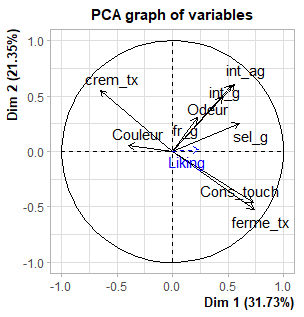
\includegraphics[scale=0.5]{pca_na_var.png}
\end{center}
\end{subfigure}~
\begin{subfigure}{0.5\textwidth}
\begin{center}
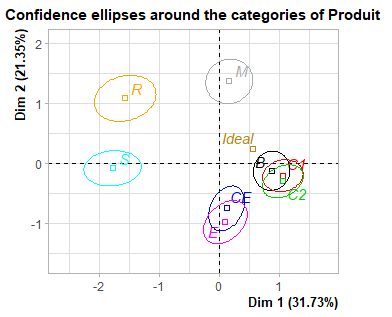
\includegraphics[scale=0.5]{pca_na_ind.png}
\end{center}
\end{subfigure}
\end{figure}

\end{frame}

%------------------------------------------------
%	NEW SLIDE
%------------------------------------------------
\begin{frame}
\textcolor{nyubluedarker}{\faCogs} On peut également \textbf{agréger} les données individuelles.

\medskip


\textcolor{nyubluedarker}{\faCogs} L'ACP est alors réalisée sur les \og produits moyens \fg{}.

\medskip

\textcolor{nyubluedarker}{\faCogs} \emph{(Dans notre cas, sur les 8 \og produits moyens \fg{} + le produit fictif \og Ideal \fg{})}

\medskip

\begin{figure}
\centering
\begin{subfigure}{0.5\textwidth}
\begin{center}
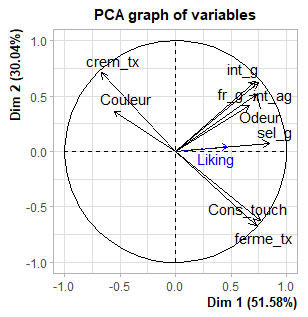
\includegraphics[scale=0.5]{pca_agg_var.png}
\end{center}
\end{subfigure}~
\begin{subfigure}{0.5\textwidth}
\begin{center}
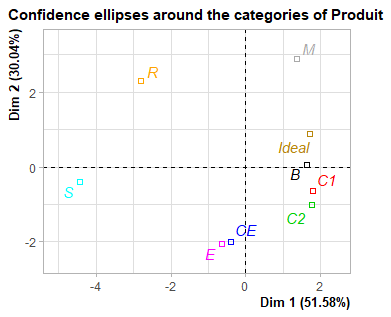
\includegraphics[scale=0.5]{pca_agg_ind.png}
\end{center}
\end{subfigure}
\end{figure}

\end{frame}

%------------------------------------------------
%	NEW SLIDE
%------------------------------------------------
\begin{frame}
	\textcolor{nyubluedarker}{\faCogs} Une telle ACP ne tient pas compte du caractère bipolaire des échelles JAR.
	
	\medskip
	
		\textcolor{nyubluedarker}{\faCogs} Par exemple, si le comté semble avoir une intensité d'arrière-goût plus faible que la moyenne des tests effectués :
			\begin{itemize}
			\item Cette intensité est-elle \og Trop faible \fg{} ?
			\item Est-elle \og Juste bien \fg{}, mais elle était trop forte pour l'ensemble des autres fromages ?  
			\end{itemize}
			
	\medskip
	
	\textcolor{nyubluedarker}{\faLightbulb[regular]} On peut re-coder les données en séparant chaque attribut en deux \emph{(dummy variables)} :
		\begin{itemize}
		\item le niveau JAR est codé 0;
		\item les valeurs 1 et 2 sont codées -1 et -2;
		\item les valeurs 4 et 5 sont codées 1 et 2.
		\end{itemize}
\end{frame}

%------------------------------------------------
%	NEW SLIDE
%------------------------------------------------
\begin{frame}
\textcolor{nyubluedarker}{\faCogs} On obtient alors un tableau comme ci-dessous.

\begin{tiny}
\begin{center}
	\begin{tabular}{lrrrrr}
  \hline
Produit & Liking & Couleur- & Couleur+ & Cons\_touch- & Cons\_touch+ \\ 
  \hline
CE & 3.00 & -1.00 & -0.00 & 0.00 & 1.00 \\ 
M & 4.00 & -1.00 & -0.00 & -1.00 & -0.00 \\ 
B & 2.00 & 0.00 & 1.00 & 0.00 & 2.00 \\ 
R & 3.00 & 0.00 & 0.00 & -2.00 & -0.00 \\ 
C1 & 4.00 & -1.00 & -0.00 & 0.00 & 1.00 \\ 
E & 1.00 & 0.00 & 0.00 & 0.00 & 1.00 \\ 
   \hline
	\end{tabular}
\end{center}
\end{tiny}

	\begin{figure}
	\centering
	\begin{subfigure}{0.45\textwidth}
	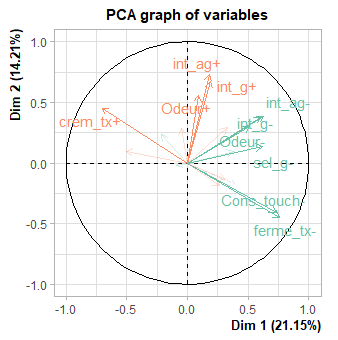
\includegraphics[scale=0.6]{var_dummy.png}
	\end{subfigure}~
	\begin{subfigure}{0.45\textwidth}
	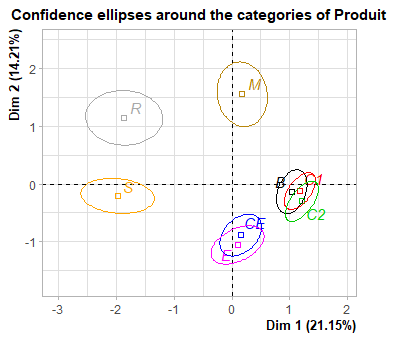
\includegraphics[scale=0.6]{ellipses_dummy.png}
	\end{subfigure}
	\end{figure}

\end{frame}

%------------------------------------------------
%	NEW SLIDE
%------------------------------------------------
\begin{frame}

\textcolor{nyubluedarker}{\faCogs} En considérant que les différentes notes sensorielles sont de nature purement \textbf{qualitative}, on peut effectuer une \textbf{Analyse des Correspondances Multiples} (ACM)

\medskip

\textcolor{nyubluedarker}{\faCogs} On retire ici la note d'appréciation globale, et on réalise l'ACM sur les $8\times 72 = 576$ données individuelles.

\medskip

\textcolor{nyubluedarker}{\faCogs} La variable catégorielle \og Produit \fg{}  est comptée ici comme une variable qualitative supplémentaire.

\begin{figure}
\centering
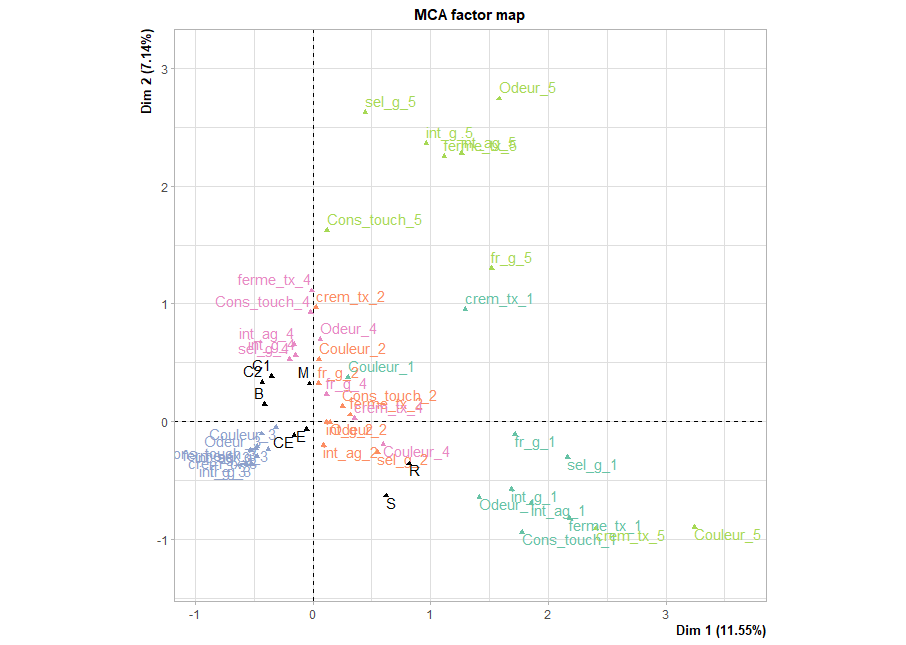
\includegraphics[scale=0.2]{mca_na.png}
\end{figure}

\end{frame}

%------------------------------------------------
%	NEW SLIDE
%------------------------------------------------
\begin{frame}

\textcolor{nyubluedarker}{\faCogs} On peut également \textbf{agréger} les données individuelles.

\medskip

\textcolor{nyubluedarker}{\faCogs} On se retrouve alors avec une table de contingence de deux variables qualitatives : \og Produit \fg{} et \og Attribut\_Note \fg{}.

	\begin{scriptsize}
	\begin{center}
\begin{tabular}{ccccccc}
  \hline
Produit & Cons\_touch\_1 & Cons\_touch\_2 & Cons\_touch\_3 & Cons\_touch\_4 & Cons\_touch\_5 & Couleur\_1 \\ 
  \hline
B &   2 &   2 &  44 &  18 &   6 &   1 \\ 
C1 &   2 &   3 &  37 &  28 &   2 &   2 \\ 
C2 &   0 &   4 &  49 &  14 &   5 &   1 \\ 
CE &   0 &   7 &  51 &  14 &   0 &   5 \\ 
E &   1 &   4 &  52 &  15 &   0 &   1 \\ 
M &   7 &  35 &  29 &   1 &   0 &   2 \\ 
R &  27 &  34 &  10 &   1 &   0 &   1 \\ 
S &  23 &  27 &  22 &   0 &   0 &   0 \\ 
   \hline
\end{tabular}
	\end{center}
	\end{scriptsize}

\end{frame}

%------------------------------------------------
%	NEW SLIDE
%------------------------------------------------
\begin{frame}

\textcolor{nyubluedarker}{\faCogs} On effectue ensuite une simple analyse des correspondances.

	
	\begin{center}
	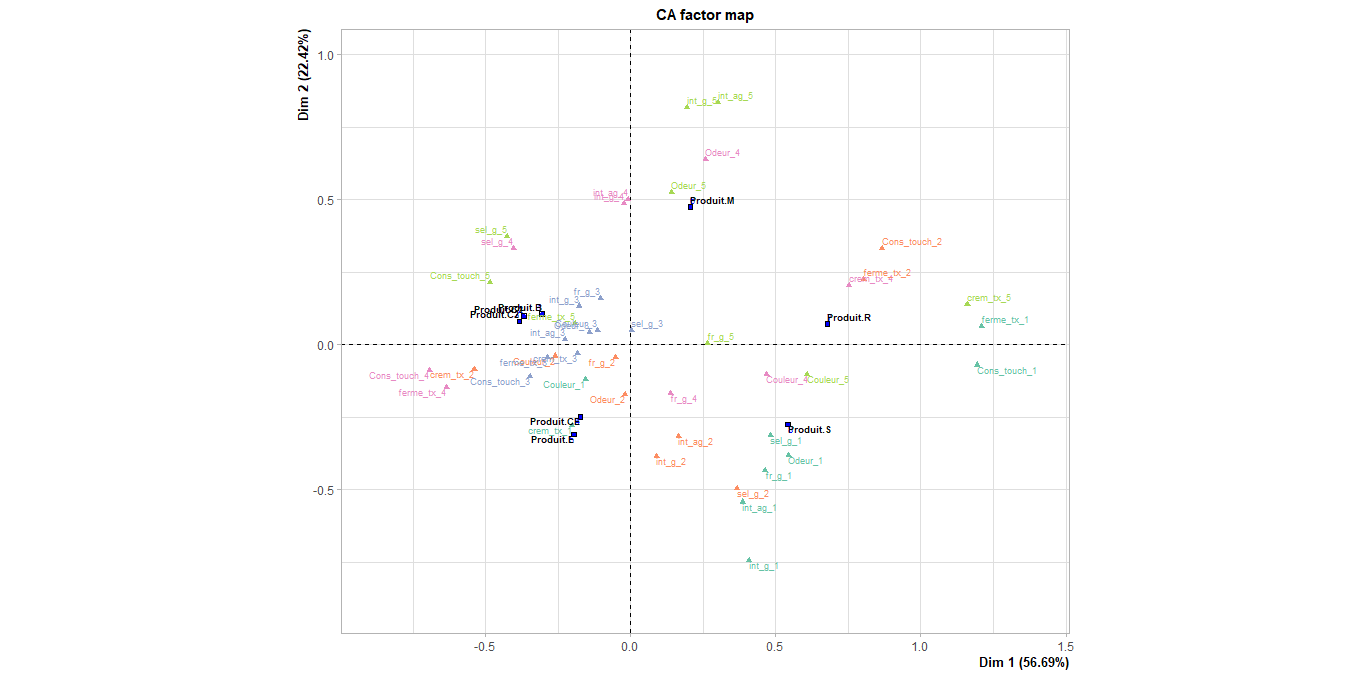
\includegraphics[scale=0.3]{ca_agg.png}
	\end{center}
	

\end{frame}

%------------------------------------------------
%	NEW SLIDE
%------------------------------------------------
\begin{frame}
	\begin{block}{\textbf{Résumé}}
		\begin{itemize}
		\item Echelle Jar = Echelle d'intensité bipolaire.
		\item Objectifs : identifier les défauts / points forts d'un produit, situer un produit par rapport aux autres.
		\item Cartographie interne.
		\item Analyse des pénalités (simple, pondérée).
		\item Analyse exploratoire : ACP, ACM, agrégation des données.
		\item Re-codage des attributs JAR en \og dummy variables \fg{} 
		\end{itemize}
	\end{block}
\end{frame}

\end{document}